% !TEX root = Projektdokumentation.tex
\section{Anhang}
\subsection{Detaillierte Zeitplanung}
\label{app:Zeitplanung}

\tabelleAnhang{ZeitplanungKomplett}

\subsection{Lastenheft (Auszug)}
\label{app:Lastenheft}

Die Anwendungen müssen folgende Anforderungen erfüllen: 
\begin{enumerate}[itemsep=0em,partopsep=0em,parsep=0em,topsep=0em]
\item Darstellung der Daten
	\begin{enumerate}
	\item Die Anwendung muss die Funktion bieten, Aufträge nach vorgegebenen Kriterien filtern zu können.
	\item Die Aufträge müssen in einer für den Planer übersichtlichen Umgebung dargestellt werden.
	\item Der Planer soll möglichst einfach und schnell Kommentare schreiben und sich anzeigen lassen können. 
	\item Der Planer soll zudem auch in den gewohnten Standardanwendungen Kommentare verfassen und lesen können 
	\end{enumerate}
\item Weitere Anforderungen
	\begin{enumerate}
	\item Die Anwendungen sollen sauber und übersichtlich programmiert werden, sodass spätere Erweiterungen leicht durchzuführen sind.
	\item Möglichst wenig Code soll in User Exits oder sonstigen Erweiterungspunkten geschrieben werden, da diese immer manuell beim Kunden eingefügt werden müssen.
	\end{enumerate}
\end{enumerate}


\clearpage

\subsection{Use Case-Diagramm}
\label{app:UseCase}
Use Case-Diagramme und weitere \acs{UML}-Diagramme kann man auch direkt mit \LaTeX{} zeichnen, siehe \zB \url{http://metauml.sourceforge.net/old/usecase-diagram.html}.
\begin{figure}[htb]
\centering
\includegraphicsKeepAspectRatio{UseCase.pdf}{0.7}
\caption{Use Case-Diagramm}
\end{figure}

\subsection{Pflichtenheft (Auszug)}
\label{app:Pflichtenheft}

\subsubsection*{Zielbestimmung}

\begin{enumerate}[itemsep=0em,partopsep=0em,parsep=0em,topsep=0em]
\item Musskriterien % Wikipedia: für das Produkt unabdingbare Leistungen, die in jedem Fall erfüllt werden müssen
	\begin{enumerate}
	\item ECC System
		\begin{itemize}
		\item Ein neues Package muss im ECC angelegt werden mit dem Namen /CAMELOT/OC.
		\item Die AUFK Datenbanktabelle muss um ein Feld mit dem Namen ZZ/\_ORDER/\_COM-MENT erweitert werden
		\item Ein extra Programm welches eine gefilterte Auswahl an Prozess-, Plan- und Produktions-Aufträgen anzeigt muss erstellt werden.
		\item Ebenfalls sollen hier jeweils die Kommentare für die Aufträge angezeigt und vom User geändert werden können. 
		\item Weiterhin soll dieses Programm massenänderungs fähig sein. 
		\item Außerdem soll es ein zweites Programm geben, in welche der User einen Tabellenfeld der AUFK Datenbanktabelle angeben kann, welches dann für die Kommentare genutzt wird.
		\item Mittels Input Checks soll verhindert werden, dass der User ein Feld angibt, dass es in der AUFK Tabelle nicht gibt
		\item Zu aller Letzt soll die COR1-3 erweitert werden.
		\begin{itemize}
			\item Ein neues Package muss angelegt werden mit dem Namen ZPP, in welches dann die COR Erweiterung kommt.
			\item Mittels der cmod Transaktion muss ein neues Projekt mit dem Namen Z\_COR angelegt werden und zwei Erweiterungspunkte hinzugefügt werden (PPCO0007 und PPCO0020).
		\end{itemize}
		\end{itemize} 
	\item APO System. 
		\begin{itemize}
		\item Es muss ebenfalls ein neues Package angelegt werden /CAMELOT/OC
		\item Die /SAPAPO/ORDFLDS muss um ein Feld mit dem Namen Order\_Comment erweitert werden.
		\item Ebenso wie im ECC System soll es ein Programm geben, welches mittels vom User eingegebener Order Number einen Auftrag mit Kommentar anzeigt, welcher vom User geändert werden kann.
		\item Desweiteren soll die RRP3 erweitert werden.
		\begin{itemize}
			\item Es muss ein neues Package mit dem Namen ZSCM angelegt werden.
			\item Mittels der se18 muss ein BAdI in diese Package implementiert werden.
			\item Die Logik muss programmiert werden.
			\item Eine implizite Erweiterung muss angelegt werden, um die T\_style Tabelle zu manipulieren.
		\end{itemize}
		\end{itemize}
	\end{enumerate}
\end{enumerate}

F
\subsection{Datenbankmodell}
\label{app:Datenbankmodell}
ER-Modelle kann man auch direkt mit \LaTeX{} zeichnen, siehe \zB \url{http://www.texample.net/tikz/examples/entity-relationship-diagram/}.
\begin{figure}[htb]
\centering
\includegraphicsKeepAspectRatio{database.pdf}{1}
\caption{Datenbankmodell}
\end{figure}
\clearpage

\subsection{Oberflächenentwürfe}
\label{app:Entwuerfe}
\begin{figure}[htb]
\centering
\includegraphicsKeepAspectRatio{MockupModules.pdf}{0.7}
\caption{Liste der Module mit Filtermöglichkeiten}
\end{figure}

\begin{figure}[htb]
\centering
\includegraphicsKeepAspectRatio{MockupModul.pdf}{0.7}
\caption{Anzeige der Übersichtsseite einzelner Module}
\end{figure}

\begin{figure}[htb]
\centering
\includegraphicsKeepAspectRatio{MockupTag.pdf}{0.7}
\caption{Anzeige und Filterung der Module nach Tags}
\end{figure}

\clearpage
\subsection{Screenshots der Anwendung}
\label{Screenshots}
\begin{figure}[htb]
\centering
\includegraphicsKeepAspectRatio{AdministrationScreenECC.png}{1}
\caption{Ändern des Feldnamens für den Kommentar in der AUFK Datenbanktabelle}
\end{figure}
\clearpage
\begin{figure}[htb]
\centering
\includegraphicsKeepAspectRatio{MaintenanceSelScreenECC.png}{1}
\caption{Selektionsbildschirm für den Maintenance Screen}
\end{figure}
\clearpage
\begin{figure}[htb]
\centering
\includegraphicsKeepAspectRatio{MaintenanceALVScreenECC.png}{1}
\caption{}
\end{figure}
\clearpage
\begin{figure}[htb]
\centering
\includegraphicsKeepAspectRatio{MaintenanceSelPopupECC.png}{1}
\caption{}
\end{figure}
\clearpage
\begin{figure}[htb]
\centering
\includegraphicsKeepAspectRatio{MaintenanceSelScreenAPO.png}{1}
\caption{}
\end{figure}
\clearpage
\begin{figure}[htb]
\centering
\includegraphicsKeepAspectRatio{MaintenanceALVScreenAPO.png}{1}
\caption{}
\end{figure}
\clearpage
\begin{figure}[htb]
\centering
\includegraphicsKeepAspectRatio{RRP3DisplayMode.png}{1}
\caption{}
\end{figure}
\clearpage
\begin{figure}[htb]
\centering
\includegraphicsKeepAspectRatio{RRP3EditMode.png}{1}
\caption{}
\end{figure}
\clearpage
\begin{figure}[htb]
\centering
\includegraphicsKeepAspectRatio{COR3.png}{1}
\caption{}
\end{figure}
\clearpage
\begin{figure}[htb]
\centering
\includegraphicsKeepAspectRatio{COR2.png}{1}
\caption{}
\end{figure}
\clearpage
\subsection{Entwicklerdokumentation}
\label{app:Doc}
\begin{center}
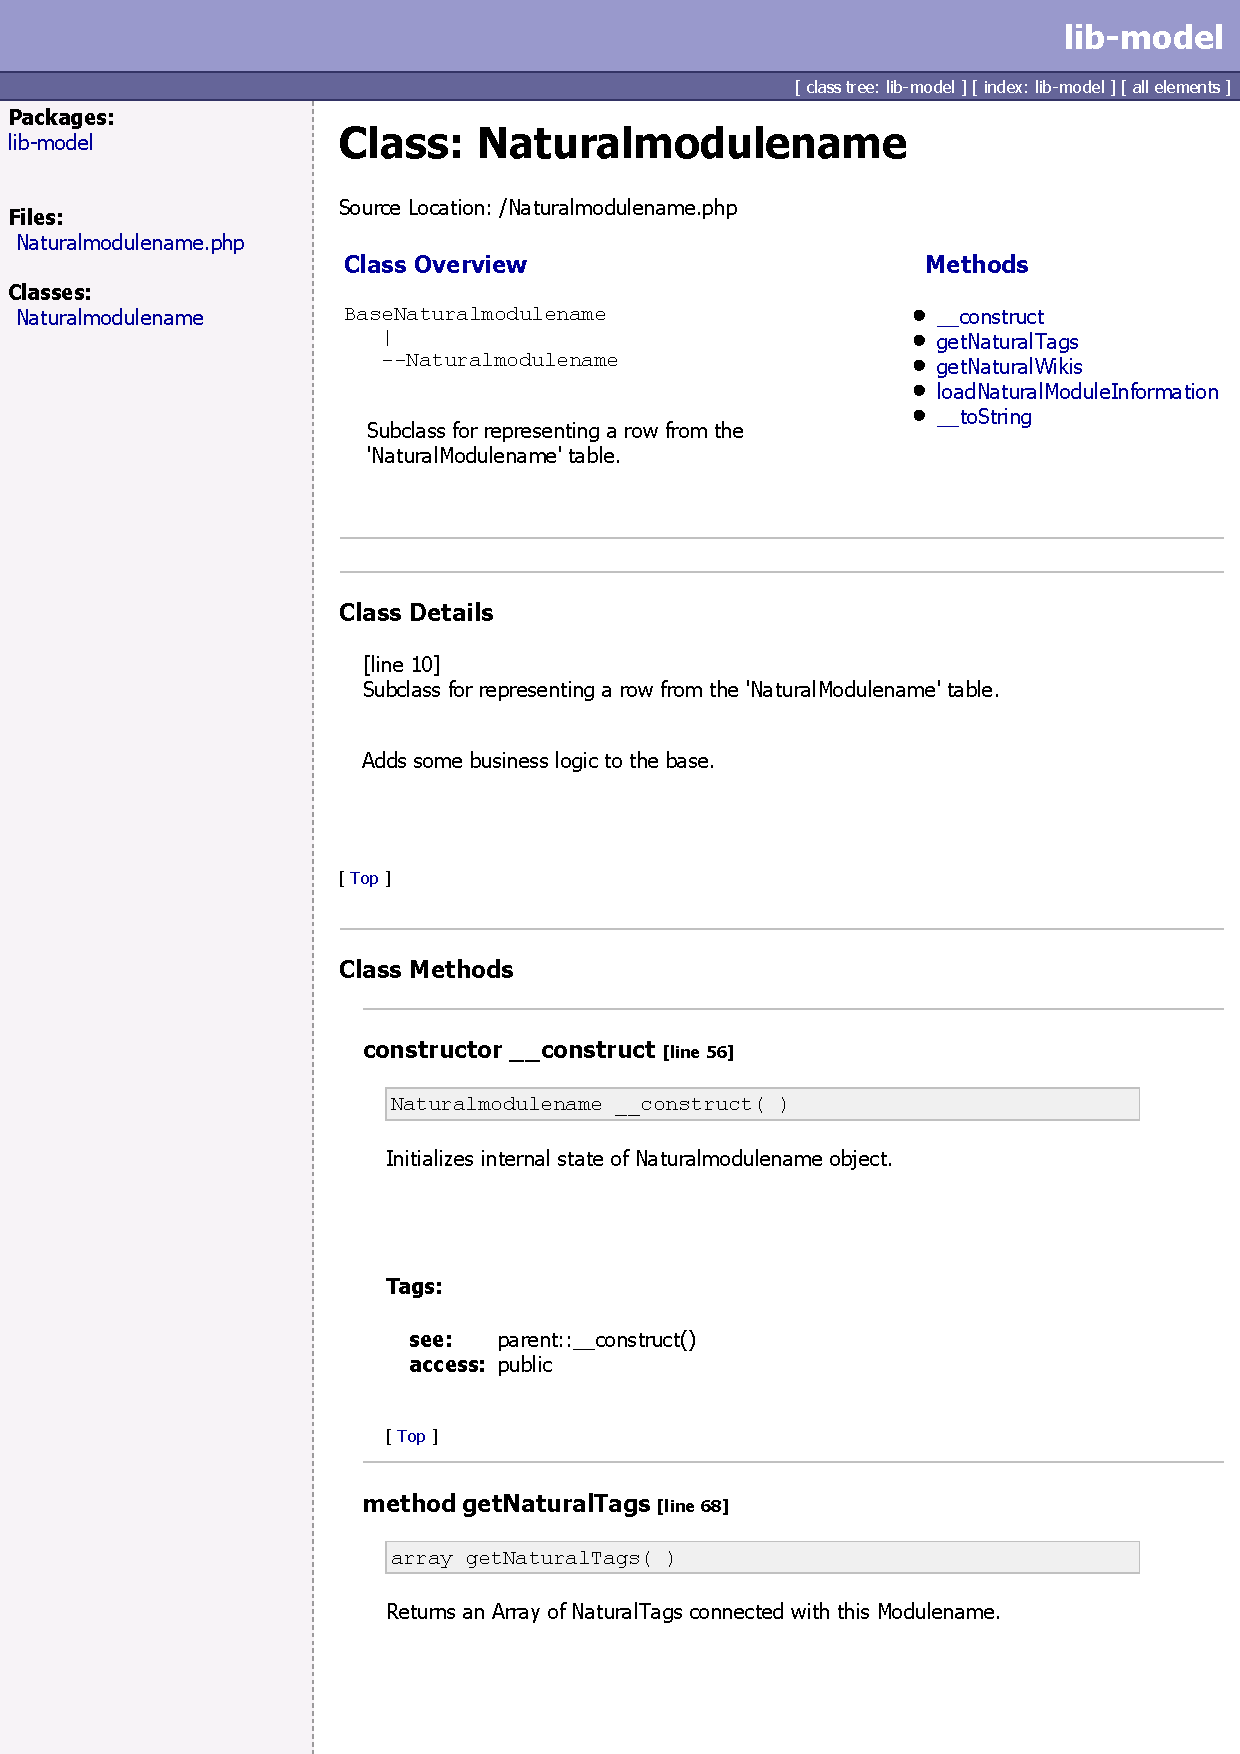
\includegraphics[page=1, width=0.9\textwidth]{doc.pdf}

\includegraphics[page=2, width=0.9\textwidth]{doc.pdf}
\end{center}

\clearpage
\subsection{Testfall und sein Aufruf auf der Konsole}
\label{app:Test}
\lstinputlisting[language=php, caption={Testfall in PHP}]{Listings/tests.php}
\clearpage
\begin{figure}[htb]
\centering
\includegraphicsKeepAspectRatio{testcase.jpg}{1}
\caption{Aufruf des Testfalls auf der Konsole}
\end{figure}


\subsection{Klasse: ComparedNaturalModuleInformation}
\label{app:CNMI}
Kommentare und simple Getter/Setter werden nicht angezeigt.
\lstinputlisting[language=php, caption={Klasse: ComparedNaturalModuleInformation}]{Listings/cnmi.php}
\clearpage

\subsection{Klassendiagramm}
\label{app:Klassendiagramm}
Klassendiagramme und weitere \acs{UML}-Diagramme kann man auch direkt mit \LaTeX{} zeichnen, siehe \zB \url{http://metauml.sourceforge.net/old/class-diagram.html}.
\begin{figure}[htb]
\centering
\includegraphicsKeepAspectRatio{Klassendiagramm.pdf}{1}
\caption{Klassendiagramm}
\end{figure}
\clearpage

\subsection{Benutzerdokumentation}
\label{app:BenutzerDoku}
Ausschnitt aus der Benutzerdokumentation:

\begin{table}[htb]
\begin{tabularx}{\textwidth}{cXX}
\rowcolor{heading}\textbf{Symbol} & \textbf{Bedeutung global} & \textbf{Bedeutung einzeln} \\
\includegraphicstotab[]{weather-clear.png} & Alle Module weisen den gleichen Stand auf. & Das Modul ist auf dem gleichen Stand wie das Modul auf der vorherigen Umgebung. \\
\rowcolor{odd}\includegraphicstotab[]{weather-clear-night.png} & Es existieren keine Module (fachlich nicht möglich). & Weder auf der aktuellen noch auf der vorherigen Umgebung sind Module angelegt. Es kann also auch nichts übertragen werden. \\
\includegraphicstotab[]{weather-few-clouds-night.png} & Ein Modul muss durch das Übertragen von der vorherigen Umgebung erstellt werden. & Das Modul der vorherigen Umgebung kann übertragen werden, auf dieser Umgebung ist noch kein Modul vorhanden. \\
\rowcolor{odd}\includegraphicstotab[]{weather-few-clouds.png} & Auf einer vorherigen Umgebung gibt es ein Modul, welches übertragen werden kann, um das nächste zu aktualisieren. & Das Modul der vorherigen Umgebung kann übertragen werden um dieses zu aktualisieren. \\
\includegraphicstotab[]{weather-storm.png} & Ein Modul auf einer Umgebung wurde entgegen des Entwicklungsprozesses gespeichert. & Das aktuelle Modul ist neuer als das Modul auf der vorherigen Umgebung oder die vorherige Umgebung wurde übersprungen. \\
\end{tabularx}
\end{table}


